\chapter{Parametric composite proposal}
\label{sec:parametric}

This chapter is a proposal of how composites could be parameterized via
an expression. With a parametric expression a composite can be reused in a
recursive way. The benefit is to create a large model without drawing all the
elements as individual components. Instead a designer creates a valid subnetwork
and set up its composite properties. In the ``large'' model the designer adds
this composite and enter its parametric expression. During parsing of the
expression the composite is called n-times, inputs and outputs are linked. The
remaining ports are those of the resulting parametric composite and need to be
connect in the model.

\paragraph{Standard concept}

The principle of how a composite is flattened and build to a canvas component is
shown in figure~\ref{fig:standard-composite-parsing}.

\begin{figure}[here]
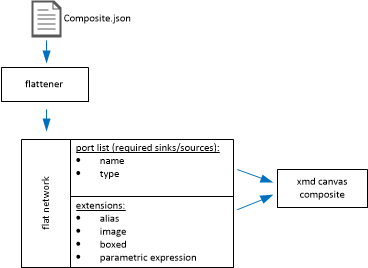
\includegraphics[width=0.75\textwidth]{pictures/composite-parsing}
\caption{standard composite parsing}
\label{fig:standard-composite-parsing}
\end{figure}

If a model is opened the flattener will request the model its composites in a
recursive way until all underlying composite are flattened. For the canvas only
the first subnetwork level is necessary to extract the required sinks and
sources.

\begin{wrapfigure}{l}{0.55\textwidth}
  \vspace{-20pt}
  \begin{center}
    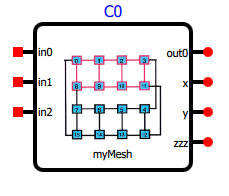
\includegraphics[width=0.20\textwidth]{pictures/composite-boxed}
  \end{center}
  \vspace{-20pt}
  \label{fig:composite-boxed}
  \caption{standard composite}
  \vspace{-10pt}
\end{wrapfigure}

Sinks and sources, marked as required, become the ports of the composite
component. The port names are the names of these sinks and sources. Sinks become
outputs while sources become inputs. The last step is to build a graphical
representation of the composite its port list and extensions. This concept is
generic and can be extended with a parametric expression. The designer tool has
already a dialog to enter the expression.

\paragraph{Parametric concept}
The propose is an expression with variable \$N which is a countdown for the
recursive function in the parametric parser. Variable \$N must be assigned to a
natural number and used as an index for network$[\$N]$ or port$[\$N]$.

A parametric expression can have three valid states:

\begin{enumerate}
\item empty : standard composite
\item \$N=n : parametric composite repeated $n+1$ times. Network and ports in
the list get index ``\$N'' where n is a natural number.
\item \$N=n , port assignments : same as in (2) but ports connected by
expression assignments.
\end{enumerate}

\begin{figure}[here]
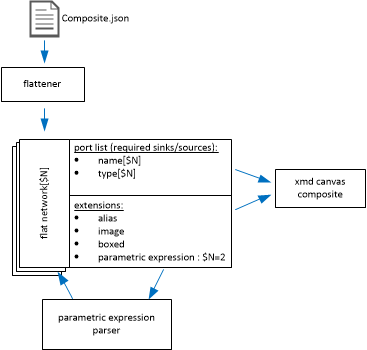
\includegraphics[width=0.75\textwidth]{pictures/composite-parametric-parsing}
\caption{parametric composite parsing}
\label{fig:parametric-composite-parsing}
\end{figure}

In the expression of figure~\ref{fig:parametric-composite-parsing}, \$N is
assigned to a value of 2. This means the flat network is duplicated two times
which result in three times the same network. Each network is added to a list at
index \$N. The same for the port list, e.g. networkX[0] its original ports ``a''
and ``b'' become $``a[0]'' and ``b[0]''$.

\begin{wrapfigure}{r}{0.30\textwidth}
  \vspace{-20pt}
  \begin{center}
    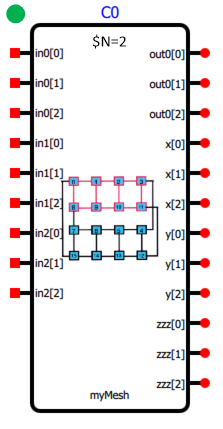
\includegraphics[width=0.20\textwidth]{pictures/parametric-composite1}
  \caption{parametric myMesh with \$N=2}
  \label{fig:parametric-composite1}
  \end{center}
  \vspace{-20pt}
\end{wrapfigure}

The result of the standard ``myMesh'' composite from the previous paragraph with
a parametric expression \$N=2 will look like
figure~\ref{fig:parametric-composite1}

The next step is the connection of ports in the expression. Suppose we want to
cascade the myMesh from figure~\ref{fig:parametric-composite1}. So that out[0]
is connected to in0[1] and so on. Only output zzz[x] is not used in the
expression and left open. The parser will start the expression with \$N=2 and
count down to zero. The expression is evaluated on each decrease of \$N.

\begin{wrapfigure}{r}{0.30\textwidth}
  \vspace{-20pt}
  \begin{center}
    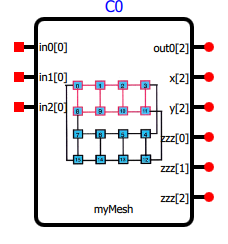
\includegraphics[width=0.20\textwidth]{pictures/parametric-composite2}
  \caption{resulting composite}
  \label{fig:parametric-composite2}
  \end{center}
  \vspace{-30pt}
\end{wrapfigure}

\begin{lstlisting}
$N=2;
if($N>0) {
   in0[$N] := out[$N-1];
   in1[$N] := x[$N-1];
   in2[$N] := y[$N-1];
 }
}
\end{lstlisting}


The resulting parametric composite is shown in
figure~\ref{fig:parametric-composite2}. The parametric parser has connected the
inner ports.

Finally we show a more complicated use of parametric composites. In the example
the expression for a spidergon is set up with 8 nodes. The composite has 3
inputs named a,b and c, and 3 outputs named x,y and z. Every node is connected
to its neighbor node clockwise and counter clockwise. Each crossing pair has
also a connection in both directions. The result is a parametric composite with
no open ports left. In the designer this can be showed as a boxed composite with
a symbol but without ports.

\begin{lstlisting}
$N=8;
if($N>=0 && $N<8) {
   a[$N] := x[$N+1]; 
   b[$N] := y[$N-1 + 8 \% 8];
   c[$N] := z[$N + (8/2) \% 8];
 }
}
\end{lstlisting}

In a similar way this can be done for a 2D mesh or whatever the expression is,
as long if its valid.

The parser must check if a port is not set more as once. This can be done in the
same way as for the canvas. If the parser asks to connect a port , but the port
is already connected the expression is invalid.



\newpage
